% !TEX root = ../main.tex

\section{Experimenty}
\label{sec:experimenty}

Ako bolo spomenuté v~predchádzajúcej kapitole, rýchlosti kolies sa dajú získať z~enkóderov. Tieto dáta sa posielajú v~správe, ktorá pripomína JSON formát.
Z~týchto vzoriek poslaných robotom nevieme priamo vypočítať polohu. Musíme si tieto dáta premeniť z~impulzov za~sekundu \(\frac{1}{s}\) na~metre
za~sekundu \(\frac{m}{s}\). Tento prevod nebude jednoznačný, pretože každý z~enkóderov posiela dáta inak zašumené. Preto~je potrebné zistiť, ako sa zmení
rýchlosť pri~zmene impulzov za~sekundu. Tento prevod (sklon prelozenej linearnej regresie cez~namerané data) je možné získať z~merania, kde~po~nastavení
rýchlostí zoberieme veľa dát z~enkóderov a~zistíme, ako sa zmení rýchlosť pri~zmene impulzov za~sekundu.

Prvý nápad na~získanie čo najlepšej prevodovej charakteristiky bolo cez~všetky dáta položiť lineárnu regresiu. To~sa ukázalo ako zlé riešenie, lebo dáta,
ktoré dostávame majú veľmi veľký rozptyl. Jednou z~nasledujúcich úvah bolo spraviť kĺzavý priemer. Toto riešenie malo tiež svoje chyby a~to~v~tom, že~zmeny
zaznamenaných impulzov za~sekundu sa zmenili v~závislosti od~rýchlosti a~smeru Obr.~\ref{fig:rw_lw_nf}. V~tomto bode sme vyskúšali počítať odometriu
z~obdržaných dát. Táto implementácia bola veľmi nepresná. Zároveň nám tento pokus potvrdil, že~potrebujeme filtrovať dáta, ktoré dostávame
od~robota, a~ktoré reprezentujú jeho rýchlosť v~impulzoch. Výsledky pokusu, kde~sme zisťovali prevodovú charakteristiku z~impulzov za~sekundu na~rýchlosť
v~SI jednotkách nájdeme na~nasledovných grafoch.

\begin{figure}[!htbp]
	\begin{subfigure}{0.5\textwidth}
		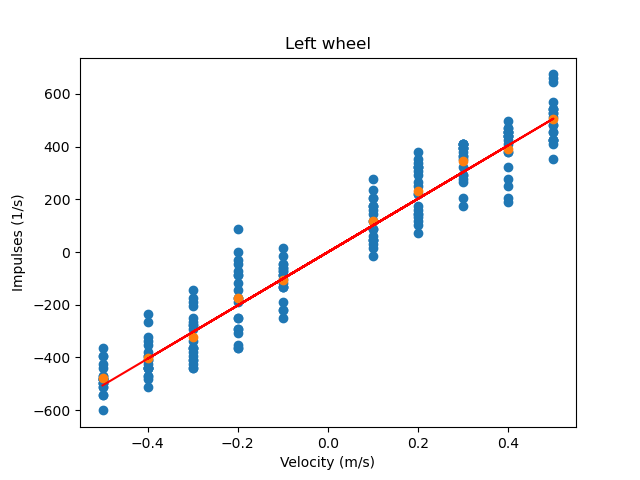
\includegraphics[width=\textwidth]{img/lw_nf.png}
	\end{subfigure}
	\hfill
	\begin{subfigure}{0.5\textwidth}
		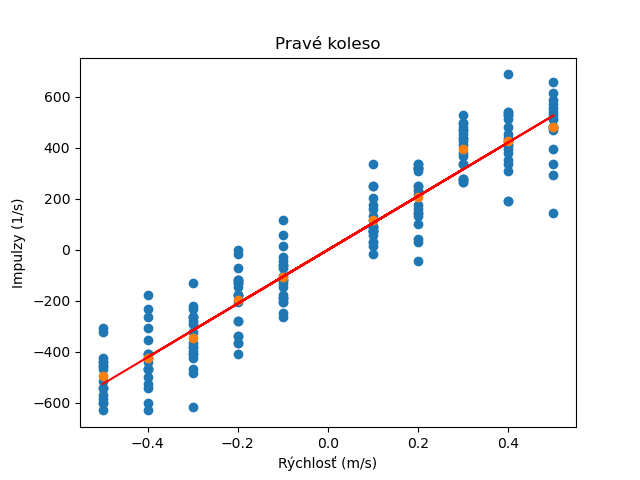
\includegraphics[width=\textwidth]{img/rw_nf.png}
	\end{subfigure}
	\caption{Získanie prevodu z~impulzov na~rýchlosť v~SI jednotkách.}
	\label{fig:rw_lw_nf}
\end{figure}

Ako prvú vec sme si vykreslili všetky \textbf{nazbierané dáta}. Tie sú~zobrazené \textbf{modrou} farbou. Cez~ne
sme spravili \textbf{lineárnu regresiu}. Je zobrazená ako \textbf{červená} úsečka. Z~nazbieraných dát sme si
nakoniec spravili aritmetický priemer, aby sme videli, ako presne aproximuje nami vypočítaná lineárna regresia priemer
nazbieraných dát. \textbf{Priemery} jednotlivých rýchlostí sú~zobrazené ako \textbf{oranžové} body.
Keď sme cez~tieto dáta polozili priamku lineárnej regresie dostali sme sklon prevodu ľavého enkóderu. Jeho
hodnota je \textbf{1012,54}. Pre~pravý enkóder to~je hodnota \textbf{1053,68}. Tento parameter
môžeme použiť v~predpočítavaní nastavenej rýchlosti robota.

Môžeme si všimnúť, že~vypočítané priemery takmer presne ležia na~vypočítanej lineárnej aproximácie. Problémom je, ako už~bolo spomenuté, že~dáta,
ktoré dostávame od~robota sú~veľmi zašumené. Preto~z~nich nevieme priamo počítať polohu robota. Na~zobrazenie veľkosti odchýlky sme spravili
meranie. Nechali sme robot aby prešiel dráhu štvorca so~stranou dlhou 1 meter a~rýchlosťou 0,5 \(\frac{m}{s}\). Výsledok bol veľmi nepresný.
Metrom sme si odmerali jeho \textit{x}-ovú a~\textit{y}-ovú súradnicu s~počiatkom v~bode, kde~sme na~robote spustili náš ovládač. Jeho skutočná
poloha bola v~bode~(-0,3m,~0m). Čo~nám ale~vypočítala odometria je, že~sa robot nachádzal 4 metre od~počiatku súradnicového systému.

\subsection{Filtrovanie zašumeného signálu}

Implementovali sme si preto~dolnopriepustný kvadratický filter. Fungovanie tohto filtra spočíva v~skombinovaní nového
vstupného parametra $\delta$ a~starého parametra $\pi_{n-1}$ uloženého vo~filtri v~danom pomere. Tento pomer je daný
parametrom \textbf{alpha} $\alpha$. Výsledok tohto výpočtu je aktuálna hodnota filtra $\pi_n$

\begin{equation}
	\pi_n = \alpha * \pi_{n-1} + (1 - \alpha) * \delta
	\label{eq:stateOfFilter}
\end{equation}

Jeho parameter $\alpha$ sme získali viacerými meraniami. Začali sme s~vysokou hodnotou filtra, $\alpha$ rovnou  0,9.

\begin{figure}[!htbp]
	\begin{subfigure}{0.5\textwidth}
		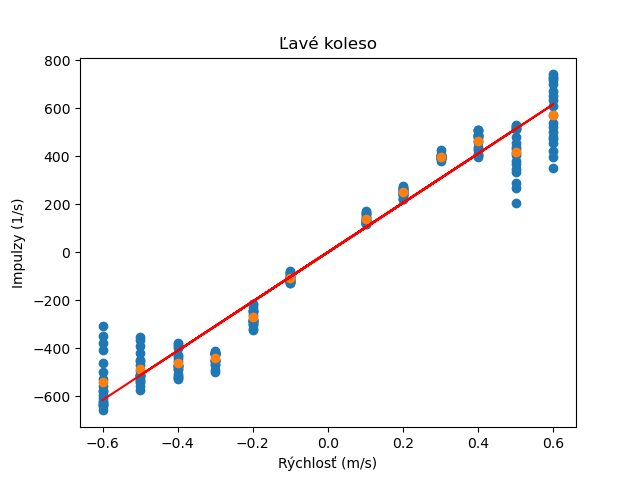
\includegraphics[width=\textwidth]{img/lw_09250.png}
	\end{subfigure}
	\hfill
	\begin{subfigure}{0.5\textwidth}
		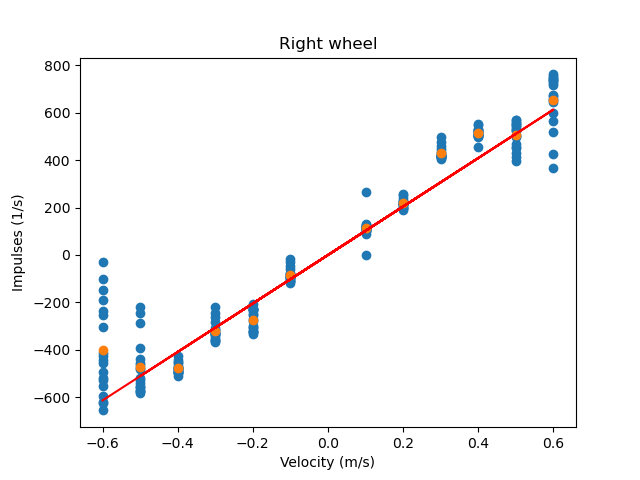
\includegraphics[width=\textwidth]{img/rw_09250.png}
	\end{subfigure}
	\caption{Získanie prevodu z~impulzov na~rýchlosť v~SI jednotkách. $\alpha$ = 0,9.}
	\label{fig:rw_lw_09250}
\end{figure}

Ako môžeme vidieť na~obrázkoch Obr.~\ref{fig:rw_lw_09250} a~Obr.~\ref{fig:rw_lw_nf} aplikácia filtra výrazne pomohla proti~šumu signálu.
Problémom pri~silnom filtri je to, že~ak~na~začiatku merania dostaneme zlú hodnotu, tak~sa táto hodnota ťažko mení na~správnu. Tento
efekt si môžeme všimnúť skoro pri~každej meranej rýchlosti. Najviditeľnejší dopad môžeme vidieť pri~pravom kolese
na~Obr.~\ref{fig:rw_lw_09250} pri~rýchlosti -0,6 $\frac{m}{s}$. Tento problém sme riešili postupným menením parametra filtru.
Aby sme predišli veľkému množstvu meraní, tak~sme použili metódy binárneho vyhľadávania.

\begin{table}
	\caption{Porovnanie výsledkov experimentov prevodu impulzov za sekundu $\frac{1}{s}$ na metre za sekundu $\frac{m}{s}$ }
	\label{tab:prevody}
	\begin{center}
		\begin{tabular}{*{4}{|c}|}
			\hline
			$\alpha$ & Frekvencia (Hz) & Ľavý enkóder & Pravý enkóder \\
			\hline
			0,9 & 250 & 1028,04 & 1021,47 \\
			\hline
			0,7 & 250 & 1126,16 & 1028,62 \\
			\hline
			0,75 & 250 & 1145,83 & 1060,25 \\
			\hline
			0,8 & 250 & 1028,81 & 1070,02 \\
			\hline
			0,8 & 100 & 1198,86 & 1212,52 \\
			\hline
		\end{tabular}
	\end{center}
\end{table}


V~tomto prípade sme začali s~veľkou hodnotou a~postupne sme skákali do~stredu nášho intervalu. Pre~toto meranie nám vyšiel
koeficient sklonu lineárnej aproximácie pre~ľavý enkóder \textbf{1028,04} a~pre~pravý nám vyšiel \textbf{1021,47} tento sklon.
Kvôli vyššie spomenutým dôvodom sme si ako ďalšiu hodnotu koeficientu $\alpha$ sme si zvolili 0,7.

\begin{figure}[!htbp]
	\begin{subfigure}{0.5\textwidth}
		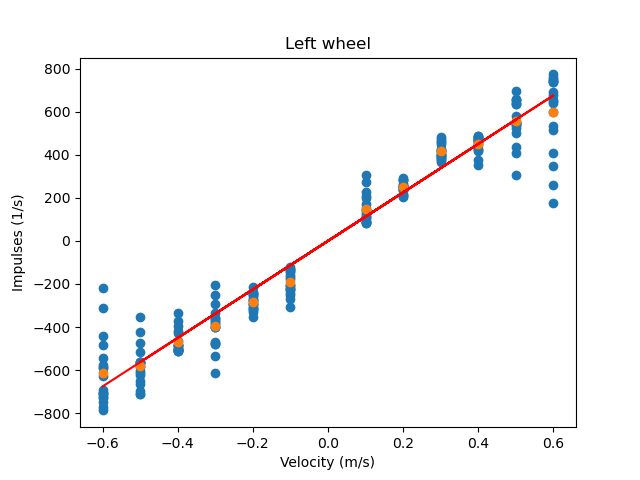
\includegraphics[width=\textwidth]{img/lw_07250.png}
	\end{subfigure}
	\hfill
	\begin{subfigure}{0.5\textwidth}
		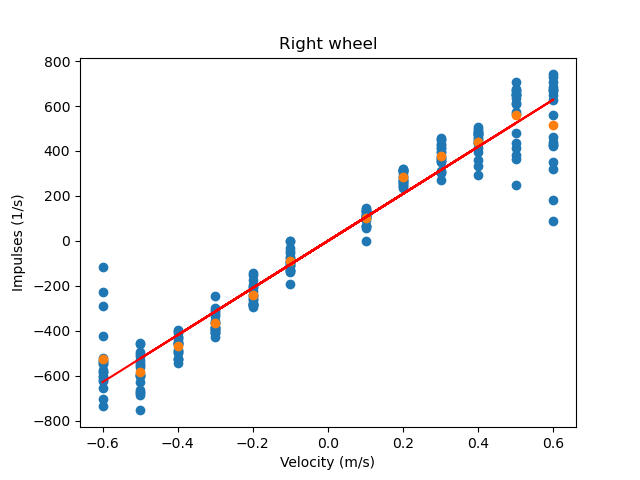
\includegraphics[width=\textwidth]{img/rw_07250.png}
	\end{subfigure}
	\caption{Získanie prevodu z~impulzov na~rýchlosť v~SI jednotkách. $\alpha$ = 0,7.}
	\label{fig:rw_lw_07250}
\end{figure}

Pri~použití koeficientu $\alpha$ s~hodnotou 0,7 (Obr.~\ref{fig:rw_lw_07250}) sme zistili, že~sa hodnoty rýchlosti aj~pri~aplikácii
filtra výrazne menili. Ustálené hodnoty zobrazené oranžovou farbou sú~podobne ako pri~meraní s~filtrom s~alphou $\alpha$
rovnou 0,9 mimo lineárnej aproximácie. Tá má sklon pre~ľavý enkóder \textbf{1126,16} a~pre~pravý enkóder to~je
\textbf{1048,62}. Neprekrytie priemeru a~aproximácie je zapríčinené iným dôvodom ako pri~silnejšom filtri. Pokým
pri~silnejšom filtri sme dostali zlú počiatočnú hodnotu, tak~už~bolo zložité ju zmeniť. Pri~slabšom filtri, ak~dostávame
rozdielne vstupné hodnoty tak~sa výstupná hodnota filtra ľahko mení. To~má za~dôsledok posun priemeru vstupných hodnôt.
Tento efekt sa dá odstrániť zosilnením filtra, čiže zväčšením koeficientu alpha $\alpha$. Spravili sme preto~ďalšie meranie,
pri~ktorom sme použili hodnotu koeficientu $\alpha$ rovnú 0,75.

\begin{figure}[!htbp]
	\begin{subfigure}{0.5\textwidth}
		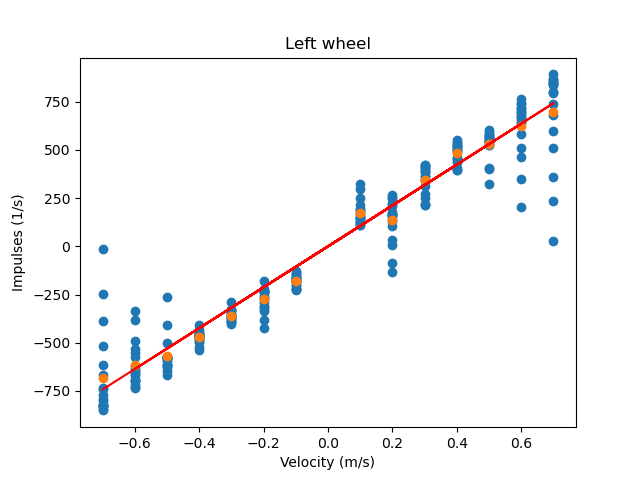
\includegraphics[width=\textwidth]{img/lw_075250.png}
	\end{subfigure}
	\hfill
	\begin{subfigure}{0.5\textwidth}
		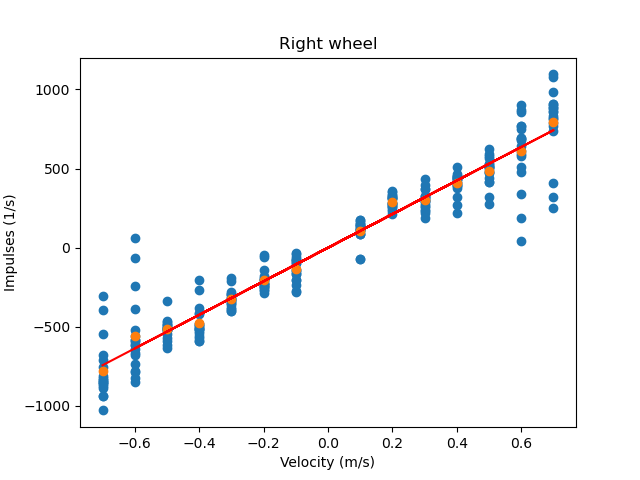
\includegraphics[width=\textwidth]{img/rw_075250.png}
	\end{subfigure}
	\caption{Získanie prevodu z~impulzov na~rýchlosť v~SI jednotkách. \(\alpha\) = 0,75.}
	\label{fig:rw_lw_075250}
\end{figure}

Obr.~\ref{fig:rw_lw_075250} zobrazuje graf výsledkov nameraných pri~aplikácii filtra s~koeficientom alpha $\alpha$ o~veľkosti
0,75. V~tomto prípade sa priemerné hodnoty na~rozdiel od~filtrov s~koeficientami alpha 0,9 a~0,7 dostali takmer priamo na~úsečku
lineárnej regresie prevodu z~impulzov za~sekundu na~metre za~sekundu. Pričom sklon aproximácie sa zmenil pre~ľavý
enkóder na~hodnotu \textbf{1145,83} a~pre~pravý enkóder je hodnota sklonu aproximácie \textbf{1060,25}. Použitie silnejšieho filtra
síce pomohlo rýchlejšiemu ustáleniu hodnoty, ale~pre~istotu sme~skúsili ešte silnejší filter s~hodnotou alpha $\alpha$ rovnou 0,8.

\begin{figure}[!htbp]
	\begin{subfigure}{0.5\textwidth}
		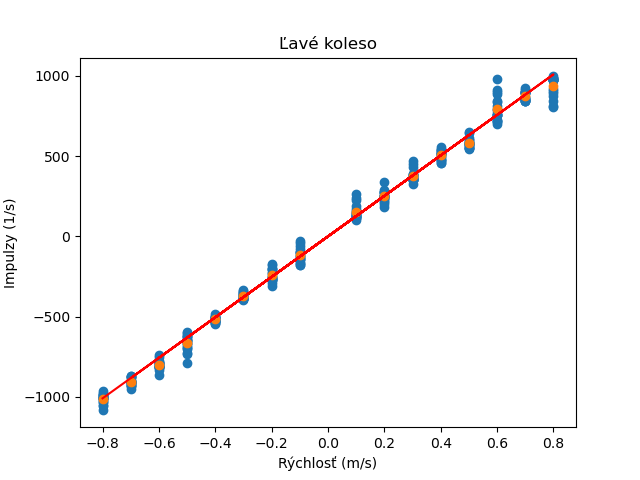
\includegraphics[width=\textwidth]{img/lw_08250.png}
	\end{subfigure}
	\hfill
	\begin{subfigure}{0.5\textwidth}
		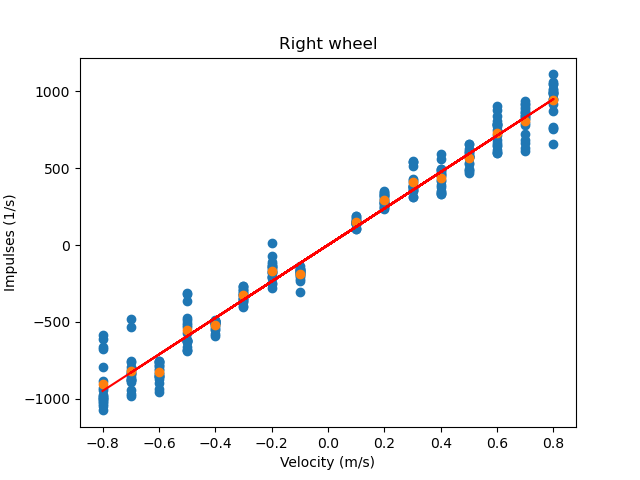
\includegraphics[width=\textwidth]{img/rw_08250.png}
	\end{subfigure}
	\caption{Získanie prevodu z~impulzov na~rýchlosť v~SI jednotkách. $\alpha$ = 0,8.}
	\label{fig:rw_lw_08250}
\end{figure}

Ako môžeme vidieť na~Obr.~\ref{fig:rw_lw_08250} ustálenie hodnôt je veľmi jednoznačné. Vybrali sme si preto~filter s~hodnotou
koeficientu alpha $\alpha$ rovnou 0,8. Zatiaľ všetky dáta čo sme merali boli s~frekvenciou 4Hz (1 vzorka za~250 milisekúnd).
Pre~presnejší výsledok sme túto frekvenciu ešte zvýšili. Z~testov robota sme vypozorovali, že~najfrekventovanejšia frekvencia,
ktorú môže robot sprostredkovať je 10Hz (1 vzorka za~100 milisekúnd). Spravili sme si preto~test na~prevod rýchlosti ešte raz
s~rovnakou hodnotou koeficientu alpha $\alpha$ rovnou 0,8, ale~s~frekvenciou 10Hz namiesto už~spomenutých 4Hz.

\clearpage

\begin{figure}[!htbp]
	\begin{subfigure}{0.5\textwidth}
		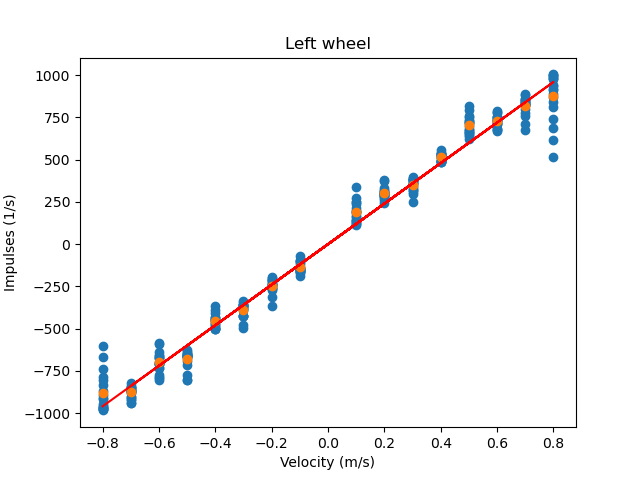
\includegraphics[width=\textwidth]{img/lw_08100.png}
	\end{subfigure}
	\hfill
	\begin{subfigure}{0.5\textwidth}
		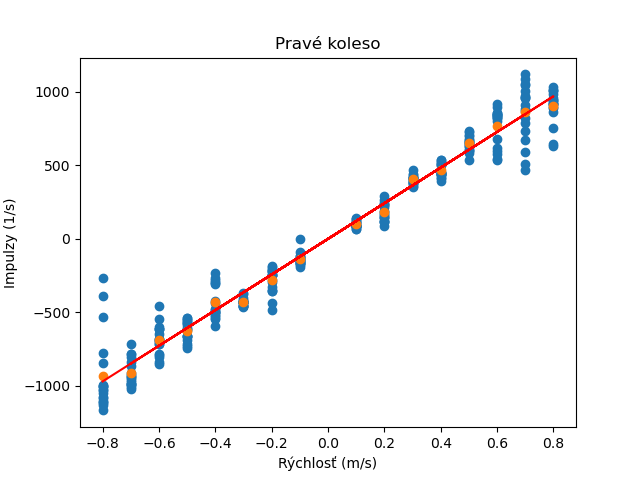
\includegraphics[width=\textwidth]{img/rw_08100.png}
	\end{subfigure}
	\caption{Získanie prevodu z~impulzov za~sekundu na~rýchlosť v~SI jednotkách. $\alpha$ = 0,8 a~frekvenciou 10Hz.}
	\label{fig:rw_lw_08100}
\end{figure}

Výsledok spomínaného merania vidíme na~obrázku Obr.~\ref{fig:rw_lw_08100}. Nie všetky získane hodnoty impulzov
z~robota sa nachádzajú pri~úsečke lineárnej aproximácie. Aj~napriek tomuto faktu sa väčšina priemerov získaných
dát nachádza na~tejto úsečke. Hodnota sklonu lineárnej aproximácie pre~pravý enkóder je \textbf{1028,81} a~pre~pravý
enkóder má aproximácia hodnotu \textbf{1070,02}. Disperzia získaných dát je chyba, ktorú odstránime ako ďalšiu.

Koeficient alpha $\alpha$ s~najlepšími parametrami nám vyšiel s~hodnotou \textbf{0,8}. Pri~implementácii tohto filtra
sme museli myslieť na~dôležitú vec. Keď sa zmenia jednorazovo impulzy na~hodnotu 0 a~hneď spať, tak~nám táto vzorka
pokazí výsledok. Musíme preto~túto vzorku ignorovať. Ďalšia prekážka, ktorú sme mali pred sebou bola zmena rýchlosti.
Obyčajná implementácia filtra by nám spomalila zmenu vypočítanej rýchlosti a~teda by spôsobila veľkú odchýlku v~polohe.
Tento problém sme opravili prestavením počiatočnej hodnoty filtra na~prvú hodnotu po~zmene rýchlosti. Toto riešenie sa
ukázalo ako najlepšie so~skúšaných riešení.

Toto riešenie má ale~jeden problém. Ak~prvá prijatá hodnota po~zmene rýchlosti nie je v~blízkom okolí žiadanej
hodnoty, tak~pôsobením filtra bude trvať dlho pokým sa hodnoty vyprodukované filtrom dostanú na~správnu hodnotu.
Tento problém vieme vyriešiť predpočítavaním hodnôt za~pomoci vypočítaných lineárnych aproximácii. Problém so~zlou
počiatočnou hodnotou môžeme vidieť aj~na~posledom grafe Obr.~\ref{fig:rw_lw_08100}. Tento problém sme vyriešili
predpočítavaním prvej hodnoty filtra po~zmene rýchlosti. Keďže sme už~mali koeficienty lineárnej regresie, tak~sme
ich využili na~predpočítanie počiatočnej hodnoty.

\clearpage

\begin{figure}[!htbp]
	\begin{subfigure}{0.5\textwidth}
		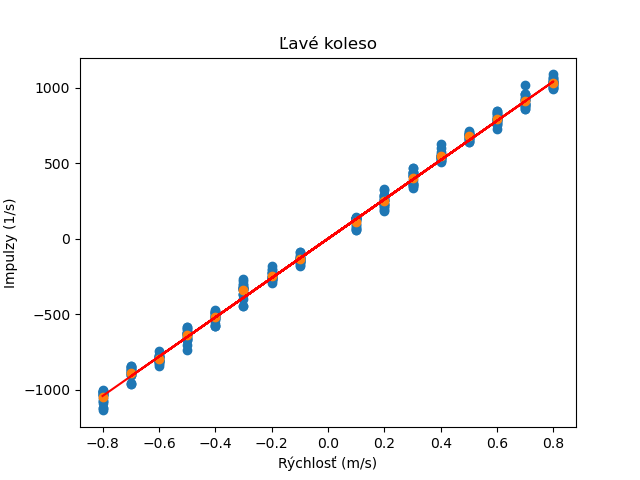
\includegraphics[width=\textwidth]{img/lw_08100_3.png}
	\end{subfigure}
	\hfill
	\begin{subfigure}{0.5\textwidth}
		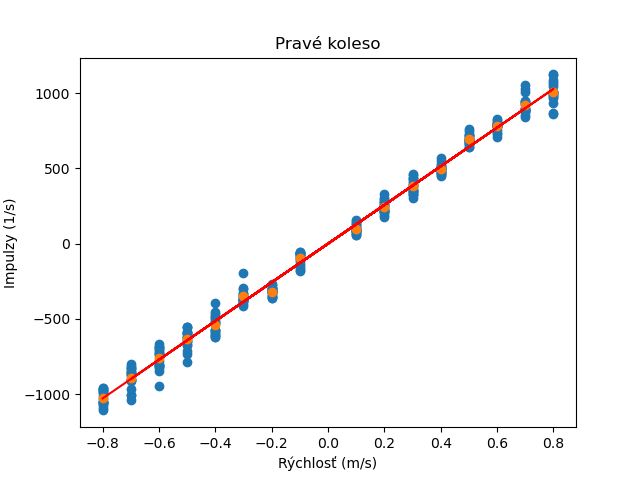
\includegraphics[width=\textwidth]{img/rw_08100_3.png}
	\end{subfigure}
	\caption{Získanie prevodu z~impulzov na~rýchlosť v~SI jednotkách. $\alpha$ = 0,8 a~frekvenciou 10Hz a~prvou prepočítanou hodnotou.}
	\label{fig:rw_lw_08100_3}
\end{figure}

Meranie so~zmenou predpočítavania prvej hodnoty sme zopakovali viackrát aby sa ustálili hodnoty aproximácie.
Po~opakovanom experimente sa nám hodnoty sklonov lineárnych aproximácii ustálili na~hodnotách:

\begin{itemize}
	\item Ľavý enkóder: \textbf{1198,86}
	\item Pravý enkóder: \textbf{1212,52}
\end{itemize}

Výsledok tohto postupu vidíme na~nasledujúcom grafe Obr.~\ref{fig:rw_lw_08100_3}.

\clearpage

\subsection{Overenie meraní}
\label{subsec:overenie_merani}

Výsledky posledných meraní filtrov sme si vyskúšali na~znázornení prejdenej dráhy v~tvare štvorca a~následne sme si
zobrazili na~grafe túto trasu. Pre~porovnanie účinnosti filtra sme porovnali tri grafy. Prvý graf zobrazuje prejdenú
dráhu počas toho ako je filter vypnutý. Druhý graf znázorňuje prejdenú dráhu s~aktívnym filtrom s koeficientom $\alpha$
rovným 0,8. Tretí graf reprezentuje dráhu prejdenú so~slabším filtrom s hodnotou koeficientu $\alpha$ 0,7.

\begin{figure}[!htbp]
	\begin{center}
		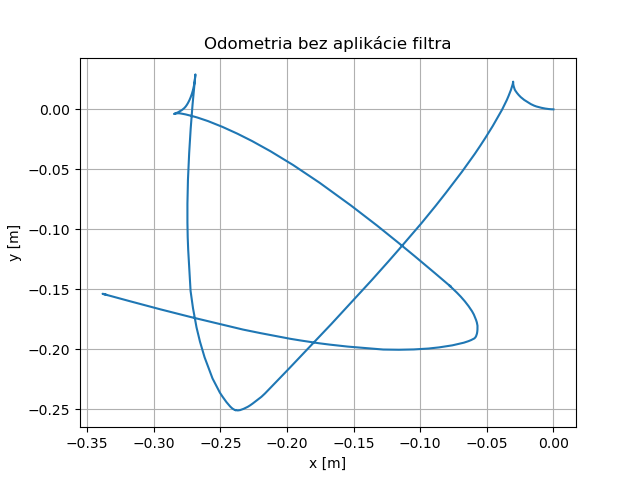
\includegraphics[width=0.8\textwidth]{img/stvorec_bez_filtra.png}
	\end{center}
	\caption{Zobrazenie pohybu robota z~odometrie bez použitia filtra.}
	\label{fig:stvorecBezFiltra}
\end{figure}

Ako prvý pokus sme vypli filtrovanie prichádzajúcich dát. To~malo za~dôsledok, že~všetky skoky, ktoré môžeme vidieť
napríklad na~obrázku Obr.~\ref{fig:rw_lw_nf} sa ukázali na~grafe. Obrázok Obr.~\ref{fig:stvorecBezFiltra} reprezentuje
dráhu, ktorú robot prešiel bez aplikácie filtra. Na~grafe môžeme vidieť zašumenie nazbieraných dát z~robota. To~sa
zobrazuje najmä v~častiach, keď má robot isť rovno. V~prípade, že~filter nepožívame, tak~rovné čiary sa premenia
na~krivky. To~spôsobuje nepresné uvedenie aktuálnej polohy. Tieto nepresnosti sa prejavujú aj~pri~otáčaní robota.
V~prípade, že~sa robot má otočiť o~90 stupňov, respektíve o~$\frac{\pi}{2}$ radiánu, tak~robot toto otočenie
reprezentuje iným uhlom, poprípade aj~posunutím.

Aby sme videli ako ovplyvňuje filter s~nami navrhnutými parametrami tak~sme spravili ďalšie meranie s~filtrom
s~najlepšími hodnotami. Druhý pokus sme zvolili najlepšiu hodnotu filtra s~koeficientom $\alpha$ rovným 0.8.
Obrázok Obr.~\ref{fig:stvorecSFiltrom} reprezentuje dráhu, ktorú robot prešiel, keď sme na~prichádzajúce dáta
aplikovali tento filter.

\begin{figure}[!htbp]
	\begin{center}
		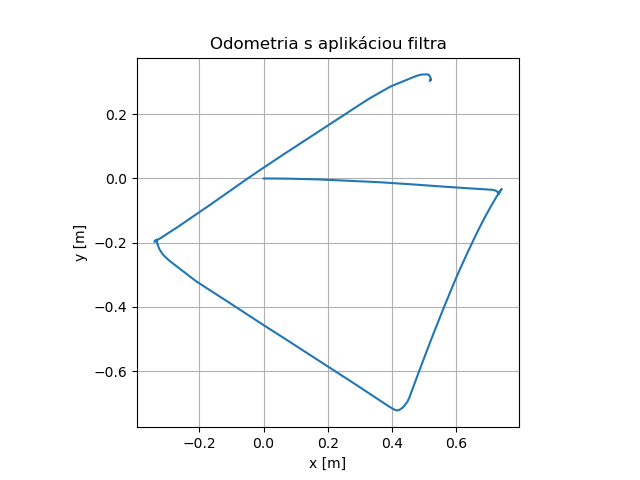
\includegraphics[width=0.8\textwidth]{img/stvorec_s_filtrom_3.png}
	\end{center}
	\caption{Zobrazenie pohybu robota z~odometrie s~použitím najlepšieho filtra.}
	\label{fig:stvorecSFiltrom}
\end{figure}

Ako môžeme vidieť na~tomto grafe tak~síce filter zlepšil výsledok, ktorý sme dostali bez filtra, ale~stále tvar, ktorý
je znázornení na~grafe nie je štvorec. Môže to~byť spôsobené viacerými faktormi.

\begin{itemize}
	\item \textbf{Prešmyk} Robot prešmykuje pri~zrýchľovaní. To~má za~dôsledok nepresné uvedenie polohy robota.
	\item \textbf{Oneskorenie komunikácie} Dáta z~ovládača prijímame vo~while cykle so~softvérovým oneskorením (100ms)
		plus \cite{timovyProjekt}. Tým, že~sa komunikácia oneskoruje, tak~sa vnáša chyba do~výpočtu aktuálnej polohy
		na~základe rýchlostí robota.
\end{itemize}

Pre~porovnanie odmeraných výsledkov odometrie a~reálneho prejdenia dráhy robotom sme odmerali vzdialenosť robota
od~začiatočnej po~konečnú pozíciu robota. Obrázky zobrazujúce toto meranie môžeme vidieť
na~Obr.~\ref{fig:stvorec_meranie_X} a~Obr.~\ref{fig:stvorec_meranie_Y}.
Odometria odmerala koniec trasy na~bod \textbf{[0,52; 0,30]}, kde~prvá hodnota zobrazuje súradnicu na~osi X a~druhá hodnota
zobrazuje súradnicu na~osi Y. Obe hodnoty boli merané v~metroch. Odmerané hodnoty metrom sme vyčíslili na~\textbf{[0,52; 0,34]}.

\begin{figure}[!htbp]
	\begin{center}
		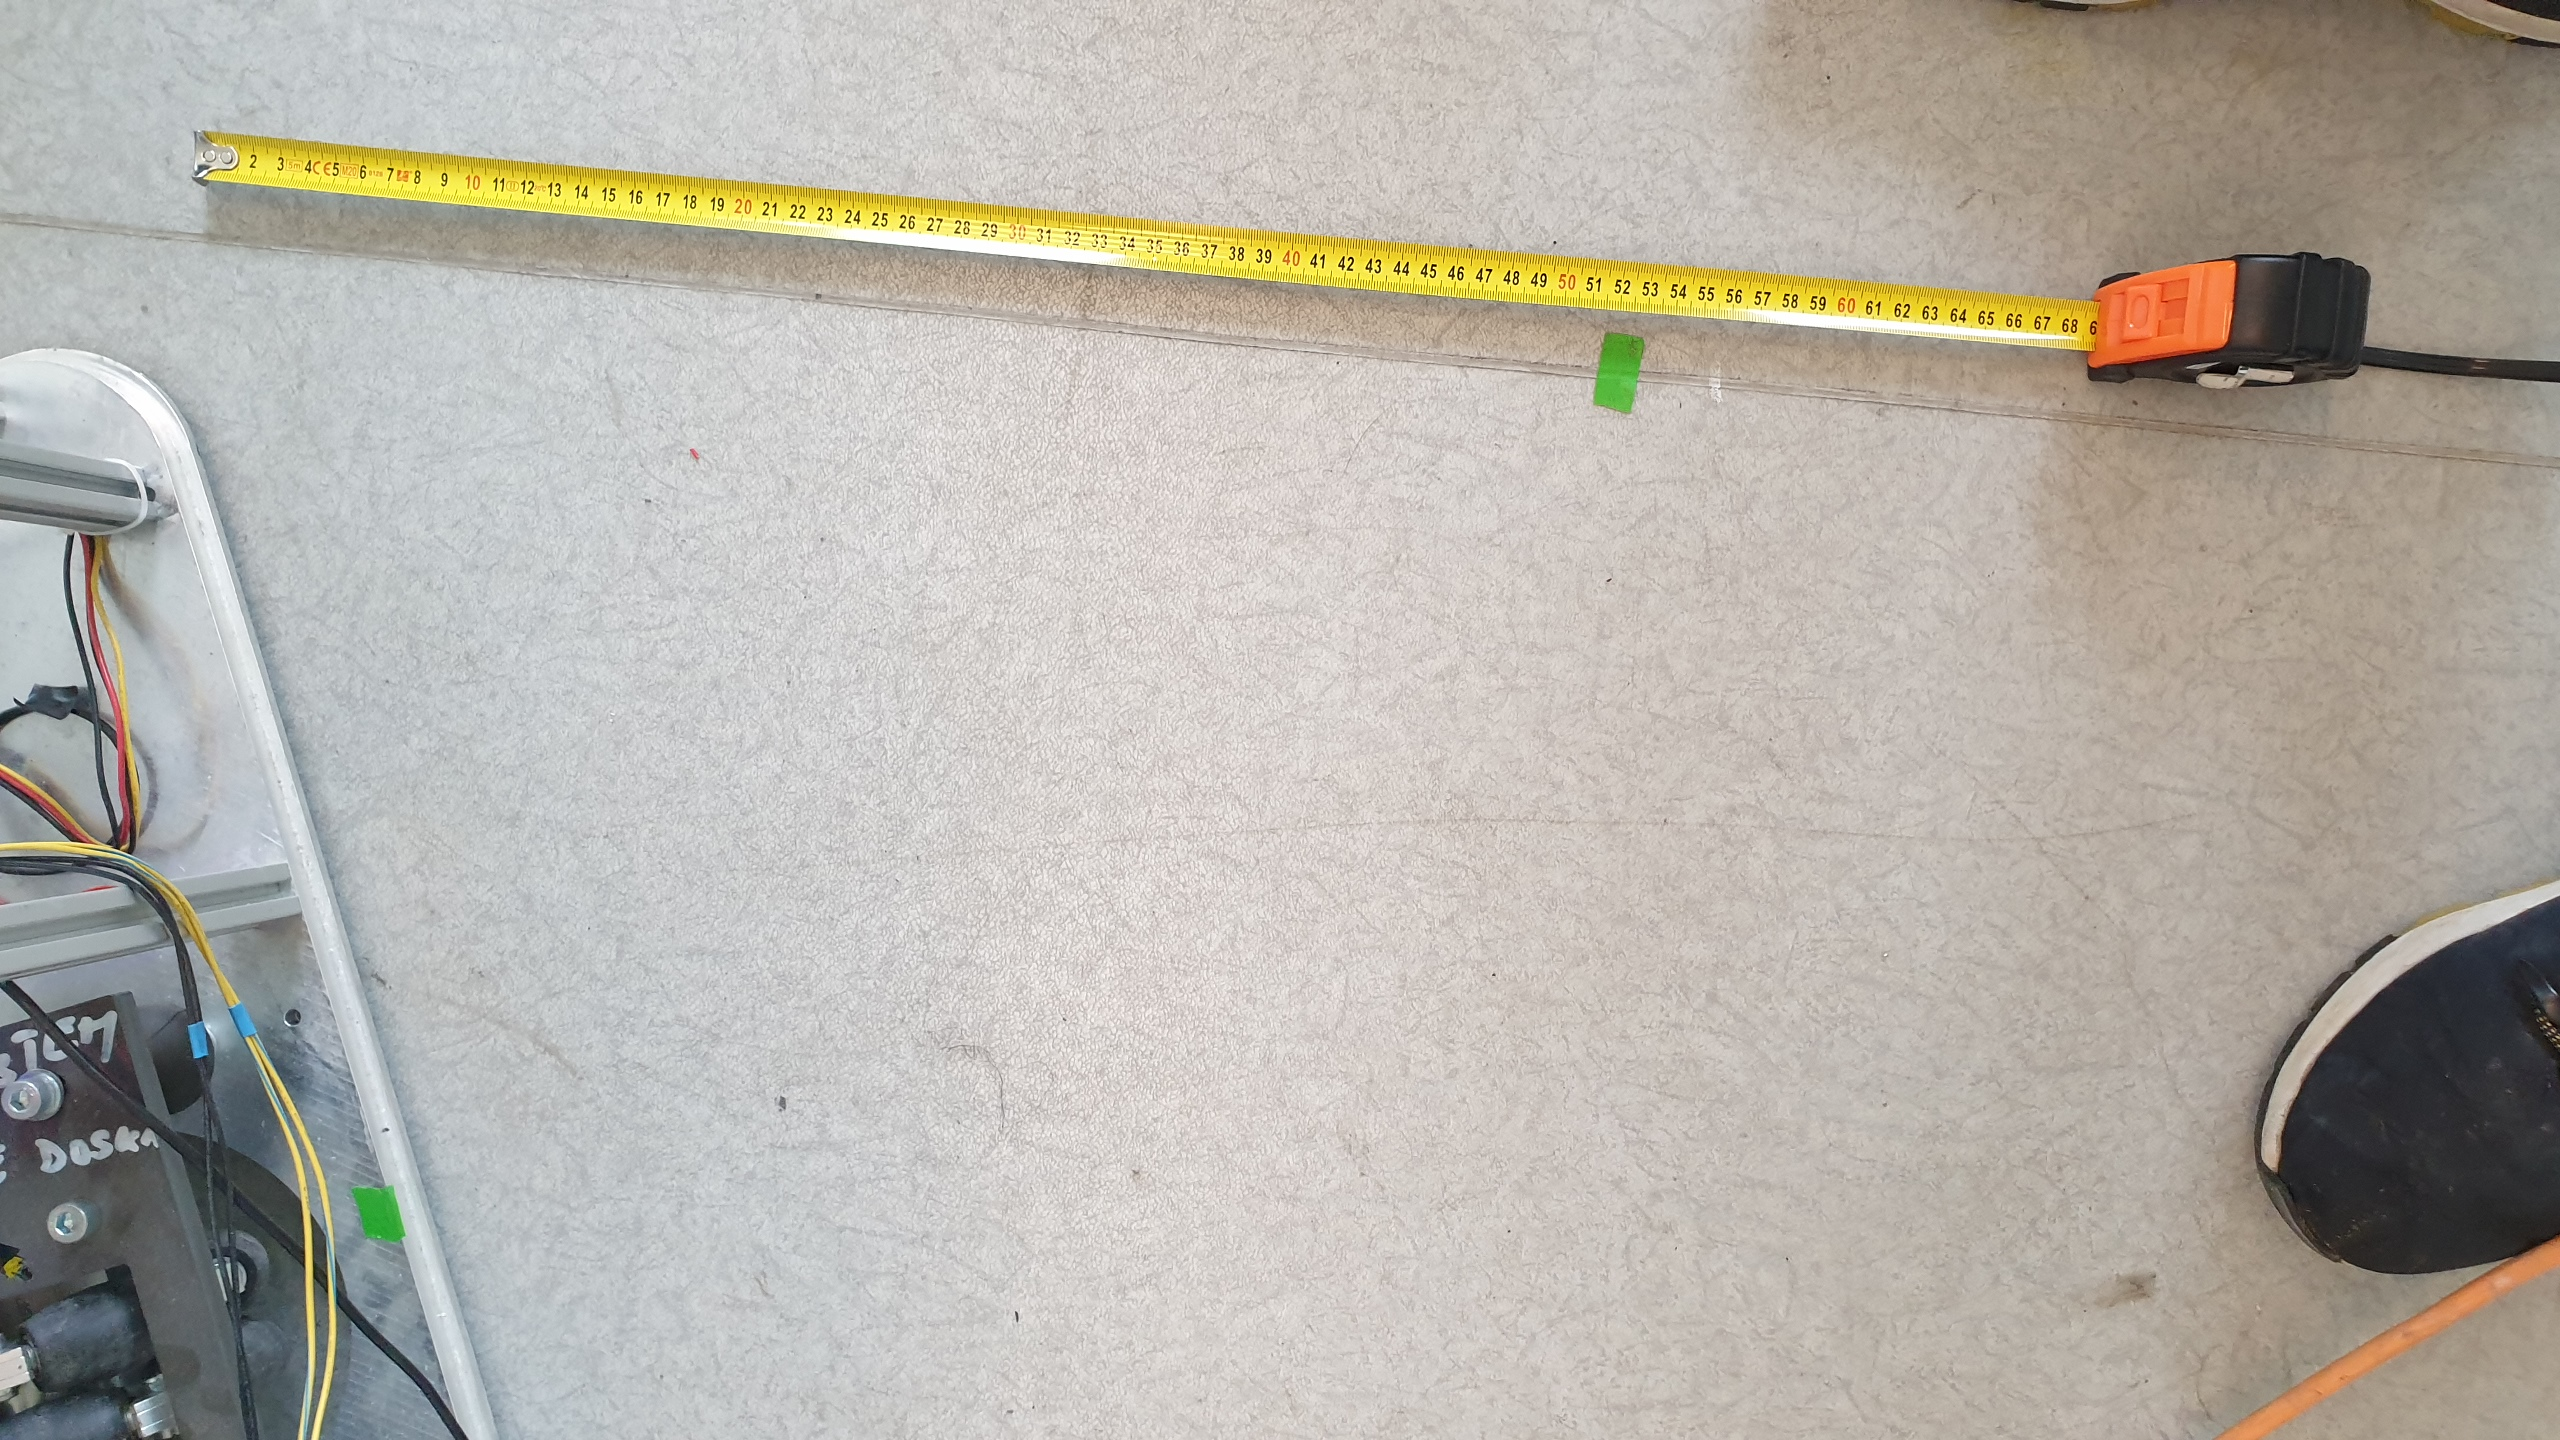
\includegraphics[width=\textwidth]{img/robot_stop_measured_X.jpg}
	\end{center}
	\caption{Odmeranie koncovej pozície robota na~osi X po~prejdení štvorcovej dráhy.}
	\label{fig:stvorec_meranie_X}
\end{figure}

\begin{figure}[!htbp]
	\begin{center}
		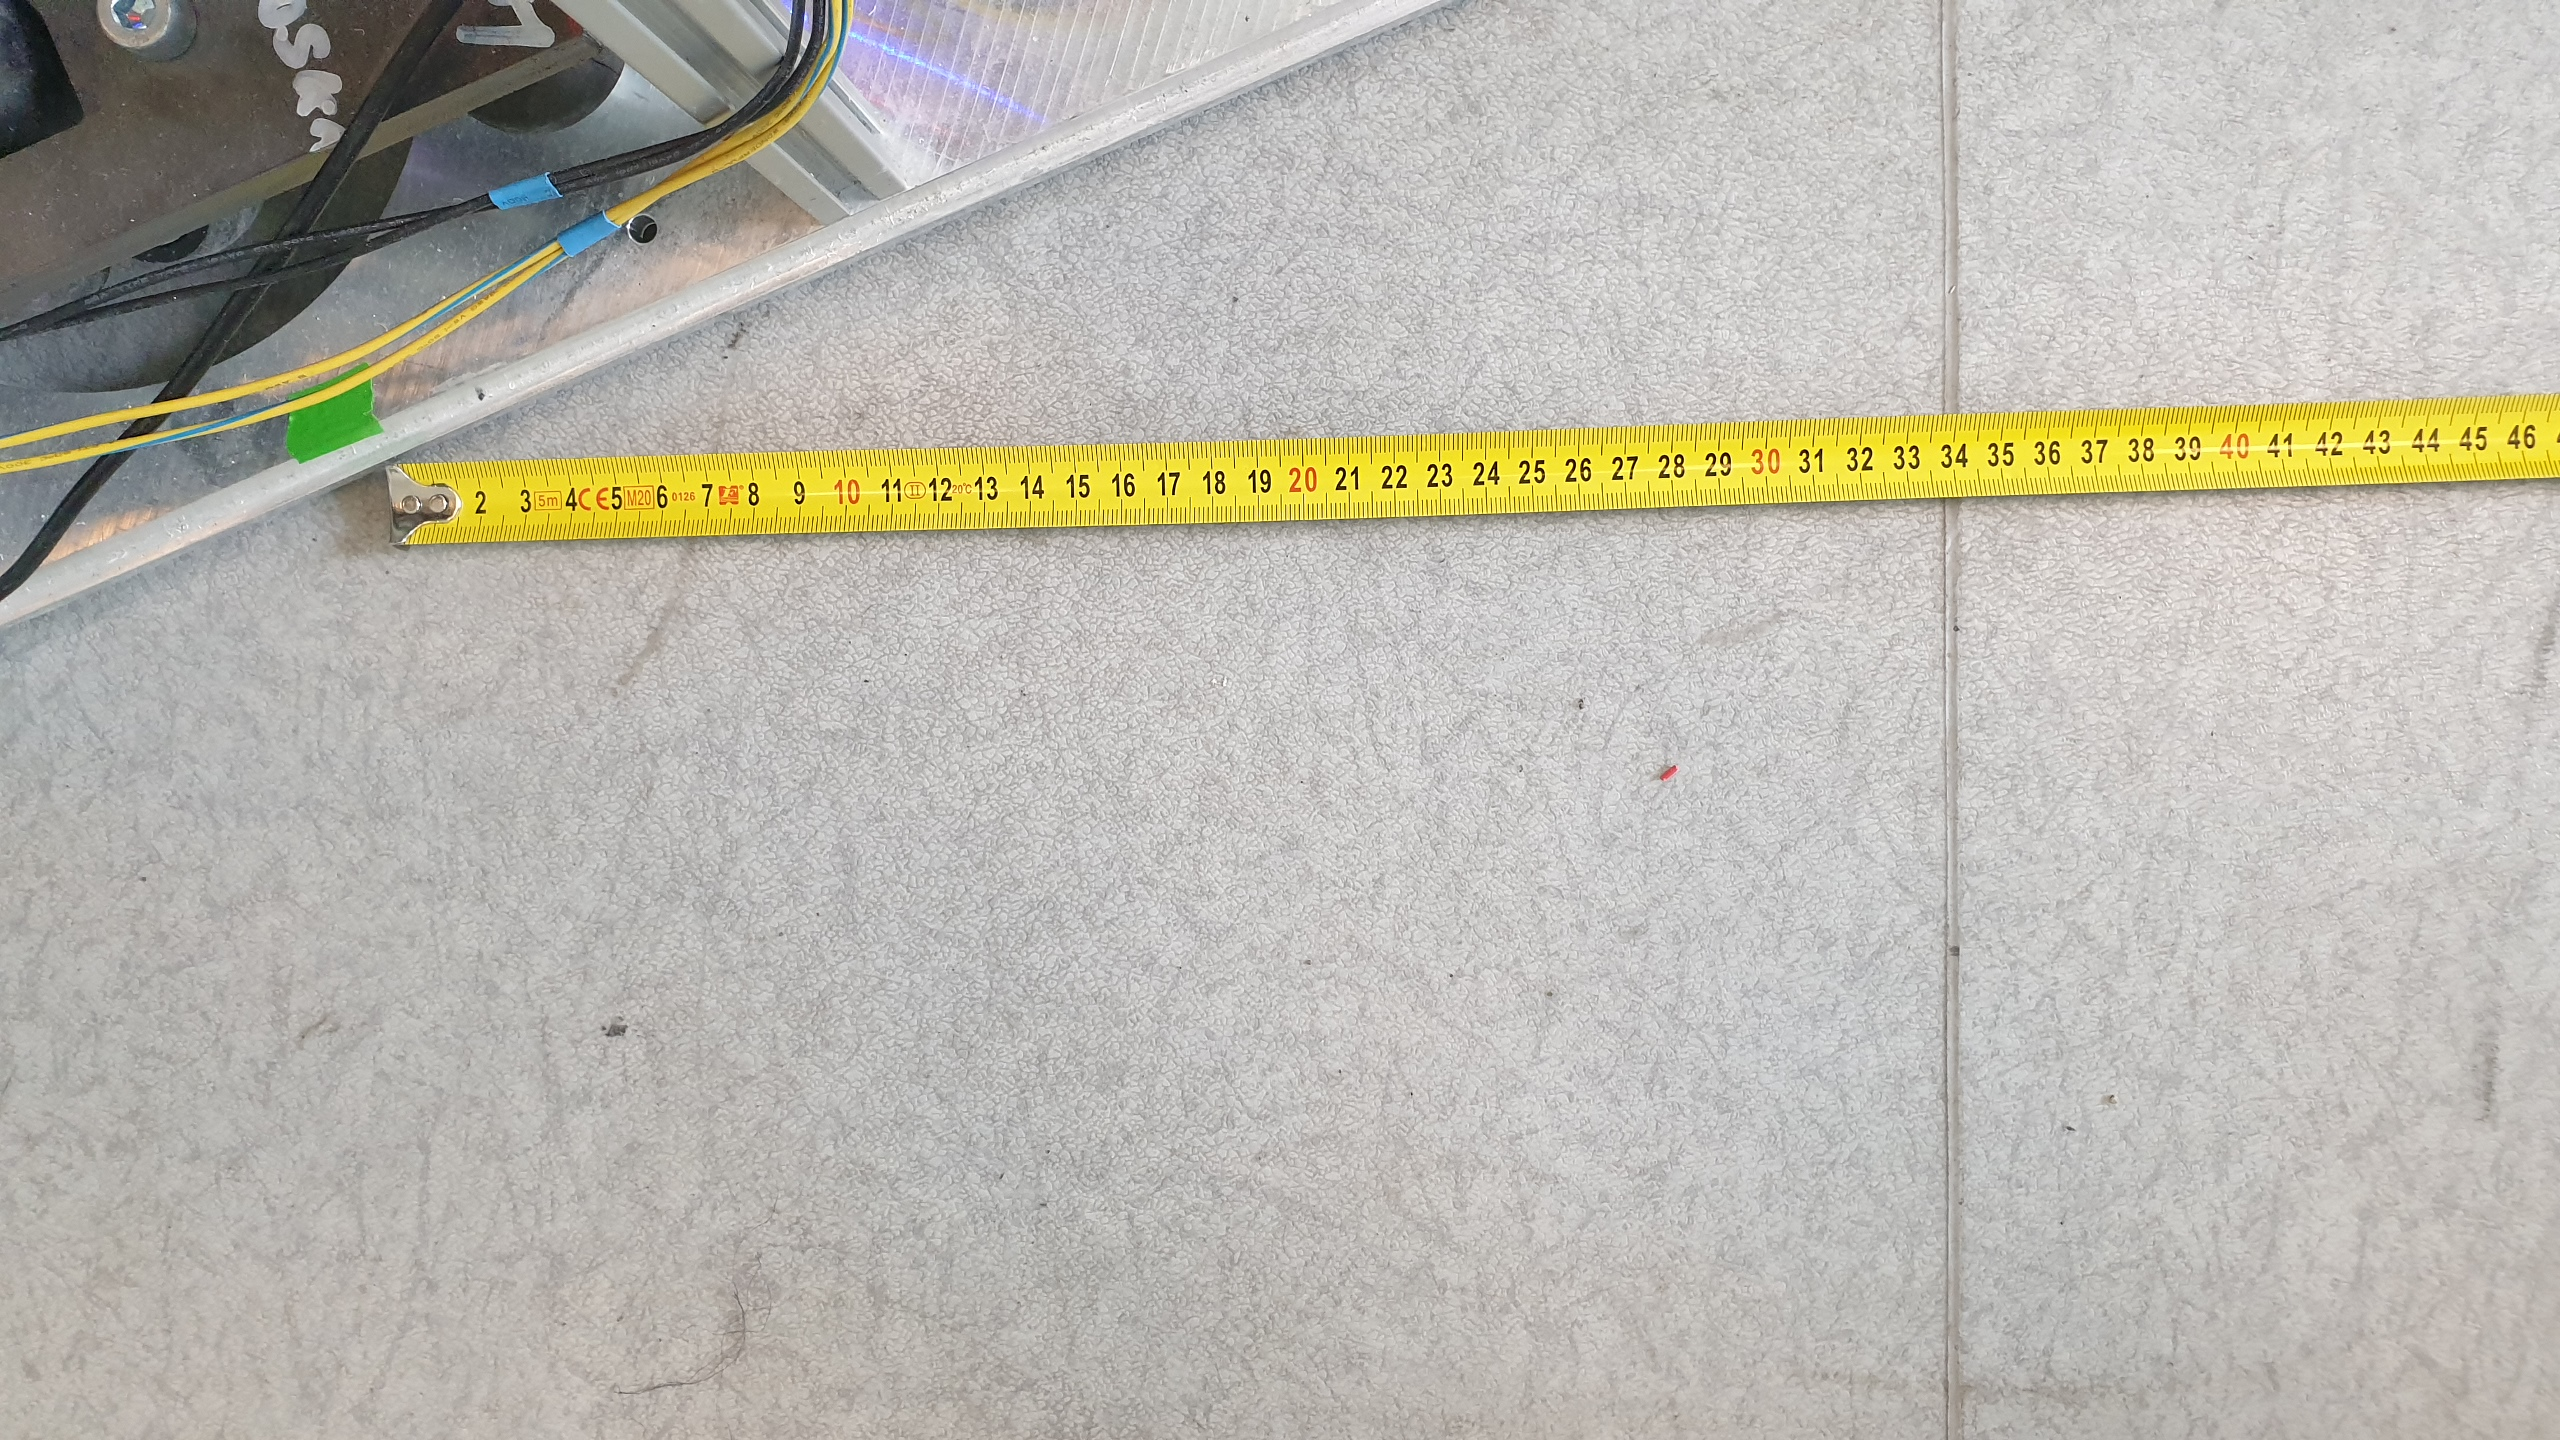
\includegraphics[width=\textwidth]{img/robot_stop_measured_Y.jpg}
	\end{center}
	\caption{Odmeranie koncovej pozície robota na~osi Y po~prejdení štvorcovej dráhy.}
	\label{fig:stvorec_meranie_Y}
\end{figure}

\clearpage

Tretie a~posledné meranie, ktoré sme spravili bolo meranie so~slabším filtrom ako sme sa rozhodli použiť. Obsahovalo
koeficient $\alpha$ s~hodnotou 0.7. Pri~takejto konfigurácii filtra sme dostali graf zobrazený na~obrázku
Obr.~\ref{fig:stvorecSoSlabsimFiltrom}. Toto zhoršenie spôsobilo slabšie filtrovanie prichádzajúcich dát a~tým pádom aj
zhoršenie presnosti určovania polohy robota.

\begin{figure}[!htbp]
	\begin{center}
		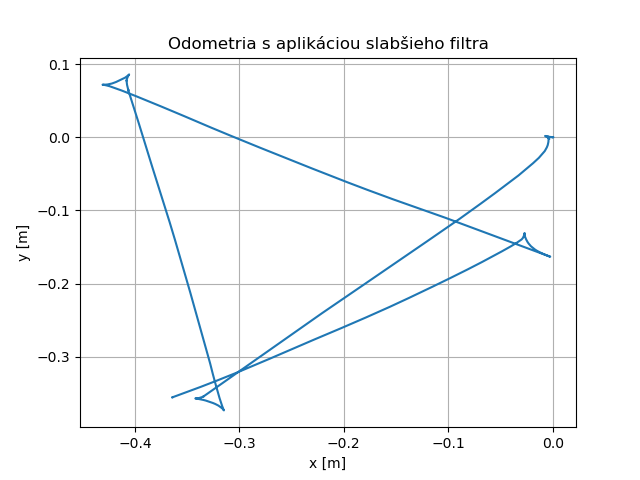
\includegraphics[width=0.8\textwidth]{img/stvorec_so_slabym_filtrom.png}
	\end{center}
	\caption{Zobrazenie pohybu robota z~odometrie s~použitím slabšieho filtra.}
	\label{fig:stvorecSoSlabsimFiltrom}
\end{figure}

Ak~by sme použili silnejší filter dostali by sme lepši výsledok. V~tom prípade by sme ale~nemali relevantný výsledok
vzhľadom na~robot. Filtrované dáta by boli až veľmi skreslené žiadanou hodnotou.

Experimentmi sme sa dostali k~najvhodnejšiemu parametru alpha $\alpha$, ktorý sme využili ako vstup
do~hodno priepustného filtra. Jeho implementáciu sme navrhli tak, aby sme vedeli zisti čo najpresnejšiu
hodnotu aktuálnych rýchlostí robota. Využitie filtra nám pomohlo presnejšie určovať aktuálnu polohu robota.


